\subsection{Morphisms of vector bundles}

7.2.1. Let B and B' be two manifolds and let f be a morphism from B to B'. Let M be a vector bundle with base B and M' a vector bundle with base B'. We say that a map g from M to M' is an f-morphism of vector bundles if the following condition is satisfied:

For every point \(b_0 \in \mathbf{B}\) , there exists a vector chart \(t = (\mathrm{U}, \varphi, \mathrm{F})\) of \(\mathbf{M}\) at \(b_0\) , a vector chart \(t' = (\mathrm{U}', \varphi', \mathrm{F}')\) of \(\mathbf{M}'\) at \(f(b_0)\) and a mapping \(\lambda\) of class \(\mathbf{C}'\) from \(\mathbf{U}\) into \(\mathcal{L}(\mathbf{F}; \mathbf{F}')\) such that \(f(\mathbf{U}) \subset \mathbf{U}'\) and that \(g_b \circ t_b = t_{f(b)}' \circ \lambda(b)\) for all \(b \in \mathbf{U}\) , where \(g_b\) is the restriction of \(g\) to \(\mathbf{M}_b\) .

Under these hypotheses, \(g\) is a morphism of manifolds and for every \(b \in B\) , \(g\) induces a continuous linear map from \(M_b\) to \(M_{f(b)}'\) . We call the rank (finite or \(+\infty\) ) of the linear map \(g_b\) the vector rank of \(g\) at \(b \in B\) , and denote it by \(\text{rg}_b(g)\) .

Conversely, if \(r \geqslant \infty\) or if \(M\) is of finite rank, an \(f\)-morphism of fibrations from \((M, B, \pi)\) to \((M', B', \pi')\) which induces on each fiber \(M_b\) a linear map from \(M_b\) to \(M_{f(b)}'\) (for every \(b \in B\) ), is an \(f\)-morphism of vector bundles.

7.2.2. Let moreover \(f'\) be a morphism of \(B'\) into a manifold \(B''\) . If \(g\) is an \(f\)-morphism of \(M\) to \(M'\) and if \(g'\) is an \(f'\)-morphism of \(M'\) into a vector bundle \(M''\) with base \(B''\) , the map \(g' \circ g\) is an \((f' \circ f)\)-morphism of \(M\) to \(M''\) . One has \((g' \circ g)_b = g_{f(b)}' \circ g_b\) for all \(b\) in \(B\) .

7.2.3. Let M and M' be two vector bundles with the same base B. One calls a B-morphism, or simply a morphism from M to M', any \(\mathrm{Id}_{\mathbf{B}}\)-morphism. The composite of two morphisms is a morphism.

Let \(g\) be a morphism of vector bundles from \(M\) to \(M'\) ; if \(g\) is bijective, it is an isomorphism of the manifold \(M\) onto the manifold \(M'\) , the inverse mapping \(g^{-1}\) is a morphism of vector bundles from \(M'\) to \(M\) and one has \((g^{-1})_b = g_b^{-1}\) for all \(b\) in \(B\) . The map \(g\) is then an isomorphism of vector bundles.

7.2.4. Let \(f\) be a morphism of a manifold \(\mathbf{B}'\) to \(\mathbf{B}\) and let \(\mathbf{M}\) be a vector bundle with base \(\mathbf{B}\) . Set \(\mathbf{M}' = \mathbf{B}' \times_{\mathbf{B}} \mathbf{M}\) and denote by \(\pi'\) (resp. \(g\) ) the restriction to \(\mathbf{M}'\) of the projection of \(\mathbf{B}' \times \mathbf{M}\) onto \(\mathbf{B}'\) (resp. \(\mathbf{M}\) ). On \(\mathbf{M}'\) there exists a vector bundle structure with base \(\mathbf{B}'\) (relative to \(\pi'\) ) and only one for which \(g\) is an \(f\)-morphism. One says that \(\mathbf{M}'\) is the vector bundle with base \(\mathbf{B}'\) inverse image of \(\mathbf{M}\) by \(f\) and is denoted \(f^* \mathbf{M}\) ; the \(f\)-morphism \(g\) is called the canonical \(f\)-morphism of \(f^* \mathbf{M}\) to \(\mathbf{M}\) .

The manifold structure of \(f^{*}\mathbf{M}\) is that of the fibered product of the manifolds \(\mathbf{B}'\) and \(\mathbf{M}\) over \(\mathbf{B}\) (5.11.2); for every \(b\in\mathbf{B}'\) , the map \(x\mapsto(b,x)\) is an isomorphism of Banach spaces from \(\mathbf{M}_{f(b)}\) onto \((f^{*}\mathbf{M})_{b}\) .

The formation of inverse images of vector bundles is transitive.

Let N' be a vector bundle with base B' and let h be an f-morphism from N' to M. There exists one and only one B'-morphism \(\tilde{h}\) from N' to \(f^{*}M\) such that \(h = g \circ \tilde{h}\) .

Let N be a vector bundle with base B and let v be a B-morphism from N to M. There exists one and only one B'-morphism, denoted \(f^{*}v\) , from \(f^{*}N\) to \(f^{*}M\) such that the diagram

\pandocbounded{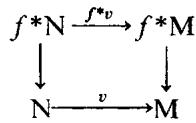
\includegraphics[keepaspectratio]{images/part001_e53c46a7.jpg}}

is commutative.

7.2.5. Let B' be a submanifold of B and let i be the canonical injection from B' into B. If M is a vector bundle with base B, the inverse image \(i^*M\) is called the vector bundle induced on B' by M and is denoted \(M|_{B'}\). If \(t = (\mathrm{U}, \varphi, \mathrm{F})\) is a vector chart of M, then \((\mathrm{U} \cap \mathrm{B}', \varphi | \pi^{-1}(\mathrm{U} \cap \mathrm{B}'), \mathrm{F})\) is a vector chart of \(M|_{B'}\). The canonical f-morphism from \(M|_{B'}\) into M is an isomorphism of manifolds from \(M|_{B'}\) onto the submanifold \(\pi^{-1}(\mathrm{B}')\) of M.

7.2.6. Let \(f\) be a morphism from a manifold B' into B and let M (resp. M') be a vector bundle with base B (resp. B'). One calls an \(f\)-comorphism from M into M' a B'-morphism from \(f^{*}M\) into M'. When B = B' and \(f = \mathrm{Id}_{\mathbf{B}}\) , the data of an f-comorphism from M into M' is equivalent to the data of a B-morphism from M into M'.

Let \(g\) be an \(f\)-comorphism of \(\mathbf{M}\) to \(\mathbf{M}'\) . For every \(b \in \mathbf{B}'\) , the map \(g_b: x \mapsto g(b, x)\) from \(\mathbf{M}_{f(b)}\) to \(\mathbf{M}_b'\) is a continuous linear map.

Additionally, let \(f'\) be a morphism of a manifold \(B''\) to \(B'\) and let \(h\) be an \(f'\)-comorphism of \(M'\) into a vector bundle \(M''\) with base \(B''\) . The map \(h \circ f'^{*}g\) of \(f'^{*}(f^{*}M) = (f \circ f')^{*}M\) to \(M''\) is then an \((f \circ f')\)-comorphism of \(M\) to \(M''\) , denoted \(h \circ g\) . For \(b \in B''\) , one has

\[
(h \circ g) _ {b} = h _ {b} \circ g _ {f ^ {\prime} (b)}.
\]

